\chapter{Questions}
% TODO: Rewrite and merge the following question/hypothesis paragraph pairs
% H1 - organization is all wrong still
The state of syntax measures in dialectometry described above leaves
several research questions unresolved. The most important for this
proposal is whether $R$ is a good measure of syntax
distance. Specifically, have the ambiguous results of previous
research been a shortcoming of $R$, differences between phonological
and syntactic corpora, or differences between phonological and
syntactic dialect boundaries?

To investigate this, I propose Hypothesis 1: the features found by
dialectologists will agree with the highly ranked features used by $R$
for classification. I will test Hypothesis 1 by comparing $R$'s
results to the syntactic dialectology literature on Swedish. In
addition, Hypothesis 1B states that the regions of Sweden accepted by
dialectology will be reproduced by $R$. For example, my
previous research on British English reproduced the well-known North
England-South England dialect regions. However, this research will eliminate the
corpus variability in that research \cite{sanders08b} that resulted in
the confounding factors mentioned above, meaning that more precise
results, such as specific identifying features, should be detectable as well.

Finally, if $R$ is found to be a bad measure of syntax distance, this
dissertation will propose and evaluate alternative syntactic distance
measures. Specifically, $R$ is one way to aggregate features that are
created by decomposing sentences. It treats features as atomic, and
does not manipulate them in any syntax-specific ways. As such, $R$ is
not much different than Goebl's WIV. This may not be a problem if the
decomposition methods used to generate features adequately capture
dialect differences in independent, atomic features. If dialect
differences cannot be captured by independent, atomic features, then a
more syntax-specific method of combining features will be needed
instead. Alternatively, a more complex statistical measure may be
useful, taking the basic idea of $R$ and increasing its
sensitivity. For example, Kullbeck-Leibler divergence, like $R$,
provides a dissimilarity that is intuitively similar to distance.

%H2 - Dad didn't understand that this is other features to be fed into
%R not replacement of R entire.
A secondary question, relevant once a useful syntax distance measure
is established, is what input features cause $R$ to produce the best
results.  Previous work has shown that leaf-ancestor paths provide a
small advantage over part-of-speech trigrams, presumably by capturing
syntactic structure higher in the parse tree. Additional possible
feature sets include variations on the previously investigated
trigrams and leaf-ancestor paths, along with various kinds of backoff,
for example, to bigrams or coarser node tags. Features from dependency
parses may be useful, too, in capturing non-local dependencies that
can be captured neither by trigrams nor leaf-ancestor paths.

Therefore, I propose Hypothesis 2: better input features
for $R$ will produce more accurate syntax
distances. These features can be discovered by comparing performance
of a number of different feature sets on a fixed corpus. In addition,
combinations of successful features will produce even better
performance.
% This sentence is either redundant or should appear earlier.
The quality of a set of features can be
measured by its sensitivity---the number of significant distances it
finds---and the similarity of the highly ranked features $R$ produces
to those found by dialectologists.

\section{Question 1 : Agreement with Dialectology}

At a high level, the first question is whether $R$, as a measure from
dialectometry, agrees with dialectology. On closer inspection, this
question covers a number of more specific questions, each dealing with
a specific comparison to dialectology. The first is whether the
features that $R$ counts most important are the same as the features
discussed in the dialectology literature. The other questions are
whether boundaries, regions and distances found by $R$ agree with
dialectology.

Feature agreement is the most important and most difficult
question. It is the most important for two reasons. First, it offers
the most precise explanation and is the easiest to disprove. Second,
dialectology starts with individual features, so the most work for
comparison is available at the feature level.

\subsection{Dialectology}

Definition of terms from dialectology is appropriate here, along with
an explanation of how they fit together. The basic unit in
dialectology is the feature, which corresponds to a feature given to
$R$. During analysis, the linguist may suspect that a feature is
characteristic of a particular region, but more information, usually
from a survey, is needed to make certain.

Given a survey or other source of geographical mapping information, a
boundary for a feature can be delineated. This boundary is called an
isogloss. With the right information, isoglosses are usually simple to
determine. One complicated case has a few occurrences of a feature
variant stranded in the middle of the other variant. This complicates
the geometry of the isogloss.

If a number of isoglosses coincide, they form an isogloss bundle,
which separates one region from another. Isogloss bundles are simple
in theory, but in practise they are difficult to find because
isoglosses rarely coincide perfectly. In practise, undisputed isogloss
bundles only occur between well-known dialects, such as the
boundaries between Low and High German or Northern and Southern
English of England. In cases where more precision is required, there
is not usually a sufficient number of coincident isoglosses. Even
though there may be plenty of isoglosses in the area, isoglosses so
rarely coincide that only a few may be construed as forming an
isogloss boundary.

Dialectology does not have a clear equivalent to dialectometry's
distance. The closest analogue is size of isogloss bundle; to reflect
this, dialect maps typically indicate size of isogloss bundle by
thickness of boundary line. Additionally, some regions are known to differ from
others much more than the rest of the regions. This usually mirrors
isogloss bundles, surfacing in the literature as a list of well-known
dialect features of a region.

\subsection{Features}

To match the features of dialectology to the features that $R$ uses to
produce a distance, I first need to find discussion of Swedish dialect
features in the dialectology literature. For example,
\namecite{rosenkvist07} discusses the South-Swedish apparent
cleft. This feature is best analysed as a single feature; Rosenkvist
mentions that it occurs in southern and central Swedish and not
northern Swedish, but does not give a more precise location than
``Svealand and G\"otaland''. So we will compare this feature directly
to features found in any part of the corpus.

Next I convert the feature to the formalism used for annotation.
Typically this requires conversion of a minimalist structure to a
simpler structure based on a phrase-structure grammar. This produces a
skeleton parse or parse fragment. Then the skeletal structure can be
broken into features in the same way that parses of corpus sentences
are. Once converted, the feature should appearch in the list of
important features for regions in southern Sweden.

In the apparent cleft example, the apparent cleft is realised as an
additional use of the word {\it som}, ordinarily a
complementiser. Typically, the next step is to identify the minimalist
structure for this, but Rosenkvist's 2007 paper does not yet provide
this analysis. Although there is no structure to translate to a
phrase-structure skeleton, his analysis provides enough clues to
produce some features directly. Trigrams are easiest; he mentions that
his corpus search used the strings {\it det \"ar som} (``It is that'')
and {\it det \"ar bara som} ``It's just that''. These words only
part-of-speech annotation to be trigram features. Dependency
paths can also use these parts of speech for the local dependencies
between {\it det,\"ar} and {\it som}. Rosenkvist also mentions
some syntactic properties of apparent clefts that are useful for
specifying dependency path features: the subject of the {\it
  som}-clause must be a pronoun, so we should expect to see
dependency paths of the form {\it ROOT-som-PRON} in the regions that
have the apparent cleft.

Once dialectometric features have been specified from some linguistic
analysis, the analysis consists of the following questions: in what
regions do these features appear? Do these regions match the expected
distribution (if any) from the linguistic analysis? How much do
the features contribute to distance from other regions? If there are
other features that contribute more, what are they?

TODO: Finish example by using structure from papers on the apparent
cleft (if it exists) in English and Japanese.

\subsection{Isogloss Boundaries}

Isogloss boundaries are intermediate in complexity between features unspecified
for location and regions demarcated by isogloss bundles. For the
purposes of this dissertation, however, there is not much difference
between a feature with some documented locations and an isogloss
boundary. An isogloss makes the regions of interest clearer, but it is
a difference in degree and not in quality. The real difference in
analysis occurs when dialectology has identified an isogloss bundle.

\subsection{Isogloss Bundles}

Isogloss bundles compare straightforwardly to dialectometry, insofar as
dialectometric methods produce regions. There are two primary ways for
identifying regions from these methods: hierarchical clustering and
multi-dimensional scaling. Neither method is perfect; as with isogloss
bundles, some human input is still needed to determine whether an
inter-region boundary truly exists at some point.

Hierarchical clustering
produces well-delineated regions, at the cost of some
uncertainty---the results tend to vary quite a bit from feature set to
feature set. Only clusters that persist between results from multiple
feature sets should be considered valid.

In contrast, multi-dimensional scaling (MDS) is a straightforward
mathematical transformation of the high-dimensional space created by
measuring distances between all regions in the corpus. Although MDS
does not produce spurious information, its results are often hard to
analyse because it produces boundaries of varying strength. Very
different regions stand out, but similar regions appear similar even
if they contain some differences. This similarity can make it
difficult to decide whether an area should be considered one region or
two.

\begin{figure}
  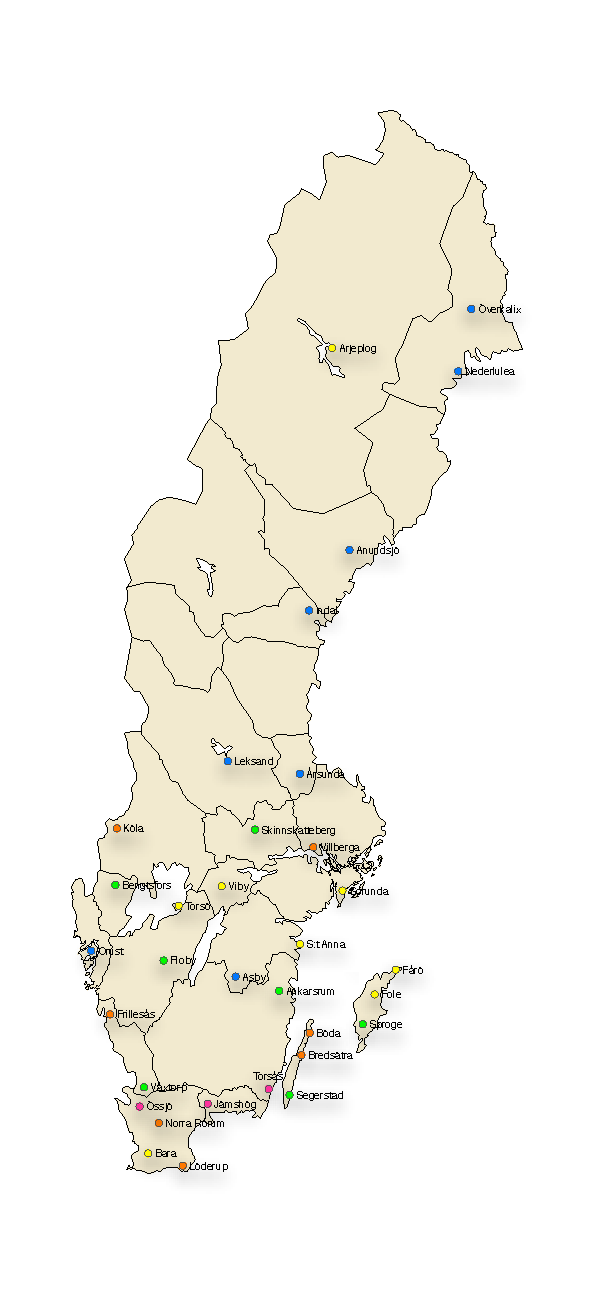
\includegraphics[width=0.32\textwidth]{Sverigekarta-Landskap-Swedia}
  \label{agree-clusters-small}
  \caption{Swedia, Clusters Common to All 3 Methods}
\end{figure}

\begin{figure}
  \includegraphics[width=0.5\textwidth]{Sverigekarta-Landskap-mds-dep}
  \label{mds-dep-small}
  \caption{Swedia, Multi-Dimensional Scaling of Depedency Path Distance}
\end{figure}

Once both dialectologic and dialectometric regions have been
identified, comparison is straightforward. Each region can be checked
for overlap---regions with a greater overlap area are better matches.

The real problem in identifying regions is that there has not been
enough dialectology work on Swedish syntax yet: numerous identified
isogloss bundles are indicative of a well understood area of
dialectology. In Swedish syntax, few regions are well-known and
well-documented enough to have isogloss bundles. It is possible that
dialectometry will lead the way in providing answers in this
area.

\subsection{Distances}

Although comparing distances from dialectometry to qualitative
research in dialectology is possible, it is unlikely to be useful in
this dissertation because of the previously mentioned lack of
developed Swedish dialectology in syntax. When it is possible,
one either looks for differences in size of isogloss bundle, or (more
weakly) statements like ``in general, Southern
Swedish is syntactically identical to Standard Swedish''
\cite{rosenkvist07} or ``there are numerous differences between
dialect X and the standard language''.

\section{Alternate Distance Measures}

Of the measures considered in this dissertation, $R$ is the
simplest---it's the sum of difference in feature counts. It is almost
the simplest statistical measure possible, given no knowledge of the
features to be used. Despite this, R appears to perform better, or
at least more consistently, than other measures that have been tested
in this dissertation. It gives significant results across a larger
variety of feature sets than more complicated measures do.

The question of measure is more important than feature set because
measures are harder to construct than feature sets, and even harder to
combine compared to feature sets. However, the distance measures
tested so far do not have a greater effect on significance also have a
greater effect on significance.


This isn't
true at the code level, but at the conceptual level, feature
sets are a lot easier to specify (copy from the proposal the 10
examples I came up with in 5 minutes).

So. Alternate distance measures. There are two directions worth
exploring: more complicated statistical measures, and more syntax
specific measures. There are more of the first and they fit more
naturally with the available data. But syntax specific measures would
be pretty cool. The problem is that most statistical syntax specific
measures can also be modelled as different feature sets, while keeping
the measure the same (more on features below).

Complicated measures are all around. WIV is one, although not really
designed for large data sets. But there are many others, like relative
entropy (Kullbeck-Leibler divergence?) and its variants
(Jenson-Shannon divergence). Probably you get could something out of
mutual information or something. I'd have to check the equation and
some commentary on it. Basically, any statistical measure of
divergence is suitable, and there don't seem to be a shortage of
those. I bet I could check Wikipedia to get a giant list that some cog
sci guys sat down and made.

\subsection{Syntax-specific distance measures}

Syntax-specific measures are harder. They have to somehow incorporate
syntax in the measure itself, in a way that can't be extracted and
reified as features for a generic measure. But this is hard for
statistical measures because syntax doesn't have much specific about
it; you have input divided into sentences, and each sentence having an
associated tree, and that's about it. Unlike phonology, you don't get
aligned words that you could use to compare the structures (trees)
directly. You don't get a well-specified several-layer model like you
do from Chomsky-Halle/Kiparsky-Archangeli.

Working by analogy from phonology, word order is equivalent to segment
order. If you want more precision than words (or better, trigrams),
model leaf-ancestor paths (and others) as bags of features for each
word. Then define a distance measure between these bags of features.

The problem with this is that, unless sentences are aligned (which
they aren't), then you'll have to compare all sentences to all
sentences. In that case any real differences will be lost in the noise
of high-distance sentences for which zero or one words match. Maybe
you could only look at sentences whose words match more than some
threshold and then compare the syntax features for each word.

\subsection{Important note on terms}

Note: divergence is a dissimilarity that is not necessarily
symmetric. Dissimilarity is a distance that is not necessarily
following the triangle inequality. I think, I should probably make
sure I'm not missing a property. Here, a ``distance measure'' really
only needs to be a dissimilarity.

\section{Question 2: Best Features}

Since the total question of this dissertation is whether syntax
distance can be made to work for dialectology, we must remember that
this is a two part question. The most important part is whether a
distance measure like $R$ can be found that works with arbitrary
features extracted from a large unaligned corpus. Once this is
established (dealt with in the previous section), the question shifts to what are
the best features.

This is an easier question, because feature sets are easier to dream
up. They are easier to combine (although I haven't done so yet.)
They are easier to tweak slightly for a great improvement in
results. The real problem with variation of feature sets is that there
no standard from syntax that can be easily adapted to
dialectometry. Phonology has order (mentioned above) and distinctive
features.

Previous work has shown that leaf-ancestor paths own a small advantage
over trigrams, and dependency paths seem to own advantages for
different measures than leaf-ancestor paths. So this question breaks
down into two pieces. How do you propose new feature sets, and how do
you tell the good ones?

\subsection{Proposing Feature Sets}

New feature sets are pretty easy to propose. Basically, chop up the
tree or dependency graph in some way, or condense the information down
in some way.  Trigrams take only the leaves, three at a
time. Leaf-ancestor paths take vertical slices of the tree. Dependency
paths take ``vertical'' slices of the graph (either arcs or nodes;
though arcs don't really work).

More lossy ways of dividing the parse might also be useful;
convolution kernels sum the differences between two trees. Oh wait, so
that wouldn't work. But something similar might. Maybe. Besides
convolution kernels, there are methods that try to identify the most
important features of the sentence manually. For example, the first or
last $n$ words in the sentence, words surrounding the predicate. Or
even lossier things like sentence length or tree height or number of
internal nodes, which captures the relative syntactic complexity of a
sentence.

Each of these has its advantages and disadvantages; leaf-ancestor
paths are good at capturing upper (hidden) structure. On the other
hand, dependency paths capture similar information but with more
emphasis on long-distance relations between words. Convolution
kernel-esque thing that I define tries to sum up the whole sentence in
a single symbol/number, as do tree height and node count. Other
specific features like first $n$ words intend to capture some aspect
of processing that will be reflected in real differences between
dialects.

\subsection{Evaluating Feature Sets}

The ideal feature set provides distances that match closely to the
real dialect differences between regions. Since these are not
precisely know, a number of proxies are necessary. One important proxy
is geographical distance; although there is no {\it a priori} reason
for geographical distance to match dialect distance, the dialectology
literature overwhelmingly shows that it does. Other proxies are
specific boundary features (mentioned above, for evaluating distance
measure). Also phonological distance.

Also, statistical significance. This is important but doesn't tell you
if you have a {\it good} set of features, only if you have a {\it bad}
set.

\subsection{Total Quality}

Total quality of the syntax distance is the multiple of distance measure
and feature set. Current results show inconsistency between measures
and sets; some combinations of measure and feature set work well, but
changing one makes it perform badly. In other words, one feature set
does not perform overwhelmingly better than the others; each feature
set has at least one measure for which it performs badly. (The
current patterns are odd.)


%%% Local Variables: 
%%% mode: latex
%%% TeX-master: "dissertation.tex"
%%% End: 
